%%%%%解析几何模版%%%%%
\chapter*{解析几何每日一题}

\refer{《高等数学》同济版}

\exercise{求过三点$M_!\qty(2,-1,4),\ M_2\qty(-1,3,-2)$和$M_3\qty(0,2,3)$的平面的方程}

\teacher{成晖}

\postdate{2023年4月17日}

\result{14x+9y-z-15}

\analysis{求过三点的平面方程，从不同的角度出发有不同的做法，下面我们一一说明}

\solutionst{
    点法式方程

    已知三点，也即知道平面上的的两个不共线向量，我们可以通过叉乘求出该平面的一个法向量，进而我们可以用点法式求解该平面方程.

    具体到这道题，由题意得
    \formula{\vv{M_1M_2}=\qty(-3,4,-6),\ \vv{M_1M_3}=\qty(-2,3,-1)}
    设平面的法向量为$n$，则
    \formula{\vv{n}=\vv{M_1M_2}\times\vv{M_1M_3}=
    \begin{vmatrix}
        \boldsymbol{i} & \boldsymbol{j} & \boldsymbol{k}\\
        -3 & 4 & -6\\
        -2 & 3 & -1
    \end{vmatrix}
    =14\boldsymbol{i}+9\boldsymbol{j}-\boldsymbol{k}
    }
    所求平面方程为
    \formula{14\qty(x-3)+9\qty(y+1)-\qty(z-4)=0,\ \mbox{即}14x+9y-z-15=0}
}

\solutionnd{三点式方程

在此之前，我们简单引入一下混合积即其运算.对于给定的三个向量$\vv{a},\ \vv{b},\ \vv{c}$，$\qty(\vv{a}\times\vv{b})\cdot\vv{c}$即为三个向量的混合积，记为$\qty(\vv{a},\vv{b},\vv{c})$.事实上，它的大小就等于以这三个向量为棱的平行六面体的体积，如下图
\begin{center}
    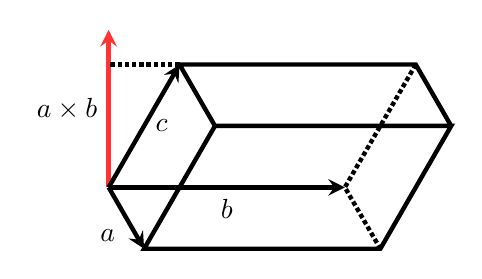
\begin{tikzpicture}
        \draw [red!80,ultra thick,-stealth] (0,0)--(0,2)node[black,midway,anchor=east]{$\vv{a}\times\vv{b}$};
        \draw [ultra thick,-stealth] (0,0)--(3,0)node[black,midway,anchor=north]{$\vv{b}$};
        \draw [ultra thick,-stealth] (0,0)--(0.9,1.56)node[black,midway,anchor=west]{$\vv{c}$};
        \draw [ultra thick,-stealth] (0,0)--(0.45,-0.78)node[black,midway,anchor=north east]{$\vv{a}$};
        \draw [ultra thick] (1.35,0.78)--(0.45,-0.78)--(3.45,-0.78)--(4.35,0.78)--(1.35,0.78)--(0.9,1.56)--(3.9,1.56)--(4.35,0.78);
        \draw [ultra thick,densely dotted] (3.9,1.56)--(3,0)--(3.45,-0.78);
        \draw [ultra thick,densely dotted] (0.9,1.56)--(0,1.56);
    \end{tikzpicture}
\end{center}

我们知道$\vv{a}\times\vv{b}$的方向与$\vv{a},\ \vv{b}$垂直，大小等于以$\vv{a},\ \vv{b}$为边的平行四边形的面积，将其视为底面面积，再将其点乘$\vv{c}$，可视为底面面积$\times$高，即平行六面体的体积.

对于混合积的运算，我们取直角坐标系$\qty{O;\boldsymbol{i},\boldsymbol{j},\boldsymbol{k}}$，设
\formula{\vv{a}=\qty(x_1,y_1,z_1),\ \vv{b}=\qty(x_2,y_2,z_2),\ \vv{c}=\qty(x_3,y_3,z_3)}
则
    \formula{
        \addtolength{\jot}{-0.5em}
        \begin{aligned}
            \qty(\vv{a}\times\vv{b})\cdot\vv{c}&=
            \begin{vmatrix}
                \vv{i} & \vv{j} & \vv{k}\\
                x_1 & y_1 & z_1\\
                x_2 & y_2 & z_2
            \end{vmatrix}\cdot
            \qty(x_3\vv{i}+y_3\vv{j}+z_3\vv{k})\\
            &=\qty(
                \vv{i}\cdot
            \begin{vmatrix}
                y_1 & z_1\\
                y_2 & z_2
            \end{vmatrix}-
            \vv{j}\cdot
            \begin{vmatrix}
                z_1 & x_1\\
                z_2 & x_2
            \end{vmatrix}-
            \vv{k}\cdot
            \begin{vmatrix}
                y_1 & z_1\\
                y_2 & z_2
            \end{vmatrix}
            )\cdot\qty(x_3\vv{i}+y_3\vv{j}+z_3\vv{k})\\
            &=x_3\cdot
            \begin{vmatrix}
                y_1 & z_1\\
                y_2 & z_2
            \end{vmatrix}-
            y_3\cdot
            \begin{vmatrix}
                z_1 & x_1\\
                z_2 & x_2
            \end{vmatrix}-
            x_3\cdot
            \begin{vmatrix}
                y_1 & z_1\\
                y_2 & z_2
            \end{vmatrix}\\
            &=
            \begin{vmatrix}
                x_3 & y_3 & z_3\\
                x_1 & y_1 & z_1\\
                x_2 & y_2 & z_2
            \end{vmatrix}=
            \begin{vmatrix}
                x_1 & y_1 & z_1\\
                x_2 & y_2 & z_2\\
                x_3 & y_3 & z_3
            \end{vmatrix}
        \end{aligned}
    }
    我们发现
    \formula{\qty(\vv{c}\times\vv{a})\cdot\vv{b}=
    \begin{vmatrix}
        x_3 & y_3 & z_3\\
        x_1 & y_1 & z_1\\
        x_2 & y_2 & z_2
    \end{vmatrix}
    =\qty(\vv{a}\times\vv{b})\cdot\vv{c}
    }
    事实上这就是混合积的轮换性.轮换混合积的三个因子，并不改变它的值，对调任意两个因子其值改变符号.
    
    下面我们推算一下三点式一般情况的求解.

    假设$P_1\qty(x_1,y_1,z_1),\ P_2\qty(x_2,y_2,z_2),\ P_3\qty(x_3.y_3,z_3)$是过平面且不共线的三点，易知$\vv{n}=\vv{P_1P_2}\times\vv{P_1P_3}$为所求平面的一个法向量，平面上任一点应满足$\vv{n}\cdot\vv{P_1P_2}=0$，即
    \formula{\qty(\vv{P_1P_2},\vv{P_1P_3},\vv{P_1P})=0}
    根据混合积公式，可得所求的平面方程为
    \formula{
        \begin{vmatrix}
            x-x_1 & y-y_1 & z-z_1\\
            x_2-x_1 & y_2-y_1 & z_2-z_1\\
            x_3-x_1 & y_3-y_1 & z_3-z_1
        \end{vmatrix}=0
}
    该式即为平面的三点式方程.

    具体到这道题，将题目中的三个点代入上式得
    \formula{
        \begin{vmatrix}
            x-2 & y-\qty(-1) & z-4\\
            -1-2 & 3-\qty(-1) & -2-4\\
            0-2 & 2-\qty(-1) & 3-4
        \end{vmatrix}=0
    }
    即该平面的方程为
    \formula{14x+9y-z-15=0}
    另外常见的求平面方法还有截距式和一般式，在面对不同问题时灵活运用即可.本期的内容到此为止啦.
}